\chapter{Categories}
\label{chap:categories}

\epigraph{
  And God saw every thing that he had made, and, \emph{behold}, it was
  very good.
}{---\textcite[Genesis 1:31]{god-1769}}

In this chapter we study categories. In Section \ref{sec:categories}
we define the concepts of category and commutative diagram, and give
several examples of categories, including the category of sets and
total functions. Besides, in Sections \ref{sec:category-haskell} and
\ref{sec:category-agda} we describe categories of types and functions
which will allow us to relate category theory to functional
programming in Haskell and Agda, respectively.

\section{Categories}
\label{sec:categories}

From the category-theoretical point of view, the concept of category
``is essentially an auxiliary one''
\parencite[247]{eilenberg-maclane-1945}. Indeed, Eilenberg and Mac
Lane defined categories in order to be able to define functors and
natural transformations. We define them in order to be able to define
everything.

\begin{definition}
  [Category]

  %% - \parencite[7--8, 10]{maclane-1998}
  %% - \parencite[418]{poigne-1992}

  %% - \parencite[1]{pierce-1991}

  \label{def:category}

  \index{category}

  A \term{category} \cat{C} consists of:
  \begin{itemize}
  \item
    \index{object}

    A set of \term{objects} \catO{C}.

  \item
    \index{morphism}
    \index{arrow|see{morphism}}

    A set of \term{morphisms} or \term{arrows} \catM{C}.

  \item
    \index{domain}
    \index{source|see{domain}}
    \index{codomain}
    \index{target|see{codomain}}

    \term{Domain} and \term{codomain} functions $\dom$ and $\cod:
    \catM{C} \to \catO{C}$, which assign to each morphism $f \in
    \catM{C}$ domain and codomain objects $a = \dom(f)$ and $b =
    \cod(f) \in \catO{C}$. We then draw an actual arrow $f: a \to b$.

  \item
    \index{identity}

    An \term{identity} function $\id: \catO{C} \to \catM{C}$, which
    assigns to each object $a \in \catO{C}$ an identity morphism
    $\idO{a}: a \to a \in \catM{C}$.

  \item
    \index{composition}

    A \term{composition} partial function $\comp\ : \catM{C} \times
    \catM{C} \to \catM{C}$, which assigns to each pair of morphisms
    $f: a \to b$ and $g: b \to c \in \catM{C}$ a composite morphism $g
    \comp f: a \to c \in \catM{C}$, that is, which assigns to each
    pair of morphisms $f$ and $g \in \catM{C}$ with $\cod(f) =
    \dom(g)$ a composite morphism $g \comp f: \dom(f) \to \cod(g) \in
    \catM{C}$. We may then draw a diagram like that of Figure
    \ref{fig:category-composition}.

    \begin{figure}[htbp]
      \begin{center}
        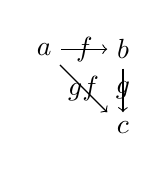
\begin{tikzpicture}
          \node (a)              {$a$};
          \node (b) [right of=a] {$b$};
          \node (c) [below of=b] {$c$};

          \draw [->] (a) to node        {$f$}         (b);
          \draw [->] (b) to node        {$g$}         (c);
          \draw [->] (a) to node [swap] {$g \comp f$} (c);
        \end{tikzpicture}
      \end{center}
      \caption{Composition of morphisms.}
      \label{fig:category-composition}
    \end{figure}

    Composition of morphisms associates to the right. Therefore, if $h
    \comp g$ and $g \comp f \in \catM{C}$, then $h \comp g \comp f$
    denotes $h \comp (g \comp f)$.

  \end{itemize}
  Additionally, the category \cat{C} is subject to the following
  axioms:
  \begin{itemize}
  \item
    \index{associativity}

    Whenever $h \comp g$ and $g \comp f \in \catM{C}$,
    \begin{equation}
      \label{eq:category-associativity}
      h \comp (g \comp f) = h \comp g \comp f = (h \comp g) \comp f
      \text{,}
    \end{equation}
    that is, the diagram in Figure \ref{fig:category-associativity} is
    commutative (see Definition \ref{def:commutative-diagram}). In
    other words, composition of morphisms is associative.

  \item
    \index{identity}

    For all morphisms $f: a \to b \in \catM{C}$,
    \begin{equation}
      \label{eq:category-identity}
      \idO{b} \comp f = f = f \comp \idO{a}
      \text{,}
    \end{equation}
    that is, the diagram in Figure \ref{fig:category-identity} is
    commutative. In other words, identity morphisms are identities for
    the composition of morphisms.

    \begin{figure}
      \begin{subfigure}[b]{0.5\linewidth}
        \begin{center}
          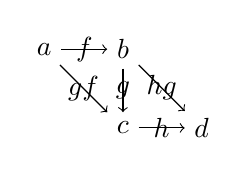
\begin{tikzpicture}
            \node (a)              {$a$};
            \node (b) [right of=a] {$b$};
            \node (c) [below of=b] {$c$};
            \node (d) [right of=c] {$d$};

            \draw [->] (a) to node        {$f$}         (b);
            \draw [->] (b) to node        {$g$}         (c);
            \draw [->] (c) to node [swap] {$h$}         (d);

            \draw [->] (a) to node [swap] {$g \comp f$} (c);
            \draw [->] (b) to node        {$h \comp g$} (d);
          \end{tikzpicture}
        \end{center}
        \caption{The associativity axiom.}
        \label{fig:category-associativity}
      \end{subfigure}
      \begin{subfigure}[b]{0.5\linewidth}
        \begin{center}
          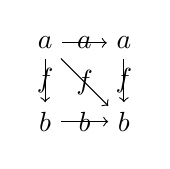
\begin{tikzpicture}
            \node (a1)               {$a$};
            \node (a2) [right of=a1] {$a$};
            \node (b1) [below of=a1] {$b$};
            \node (b2) [right of=b1] {$b$};

            \draw [->] (a1) to node        {$\idO{a}$} (a2);
            \draw [->] (b1) to node [swap] {$\idO{b}$} (b2);

            \draw [->] (a1) to node [swap] {$f$}       (b1);
            \draw [->] (a1) to node        {$f$}       (b2);
            \draw [->] (a2) to node        {$f$}       (b2);
          \end{tikzpicture}
        \end{center}
        \caption{The identity axiom.}
        \label{fig:category-identity}
      \end{subfigure}
      \caption{}
    \end{figure}

  \end{itemize}

\end{definition}

\epigraph{
  ``And what is the use of a book without pictures or conversations?''
}{---\textcite[13]{carroll-2004}}

\begin{definition}
  [Commutative diagram]

  %% - \parencite[8]{maclane-1998}
  %% - \parencite[434--435]{poigne-1992}

  %% - \parencite[27--28]{bird-demoor-1997}
  %% - \parencite[10--13]{pierce-1991}

  \label{def:commutative-diagram}

  \index{commutative diagram}
  \index{diagram!commutative ---|see{commutative diagram}}

  We often use diagrams consisting of objects and morphisms of a
  category, like that of Figure \ref{fig:category-composition}. Such a
  diagram in a category \cat{C} is said to be commutative, or to
  commute, when, for each pair of objects $a$ and $b \in \catO{C}$,
  any two paths leading from $a$ to $b$ yield, by composition, equal
  morphisms from $a$ to $b$. For instance, if we say that the diagrams
  in Figure \ref{fig:commutative-diagram} are commutative, we mean
  that
  \begin{equation*}
    h = g \comp f
    \quad
    \text{and}
    \quad
    g' \comp f' = g \comp f
    \text{,}
  \end{equation*}
  respectively. In this way, ``commutative diagrams are just a
  convenient way to visualize equalities of morphisms''
  \parencite[434]{poigne-1992}.

  \begin{figure}[htbp]
    \begin{subfigure}{0.5\linewidth}
      \begin{center}
        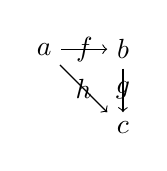
\begin{tikzpicture}
          \node (a)              {$a$};
          \node (b) [right of=a] {$b$};
          \node (c) [below of=b] {$c$};

          \draw [->] (a) to node        {$f$} (b);
          \draw [->] (b) to node        {$g$} (c);
          \draw [->] (a) to node [swap] {$h$} (c);
        \end{tikzpicture}
      \end{center}
    \end{subfigure}
    \begin{subfigure}{0.5\linewidth}
      \begin{center}
        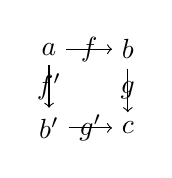
\begin{tikzpicture}
          \node (a)               {$a$};
          \node (b)  [right of=a] {$b$};
          \node (b') [below of=a] {$b'$};
          \node (c)  [below of=b] {$c$};

          \draw [->] (a)  to node        {$f$}  (b);
          \draw [->] (b)  to node        {$g$}  (c);
          \draw [->] (a)  to node [swap] {$f'$} (b');
          \draw [->] (b') to node [swap] {$g'$} (c);
        \end{tikzpicture}
      \end{center}
    \end{subfigure}
    \caption{Examples of commutative diagrams.}
    \label{fig:commutative-diagram}
  \end{figure}

\end{definition}

\begin{remark}

  %% - \parencite[434--435]{poigne-1992}

  %% - \parencite[12]{pierce-1991}

  \label{re:commutative-diagram}

  Moreover, commutative diagrams are closed under composition of
  diagrams in that a diagram commutes if all its subdiagrams commute.
  For example, if we say that the inner triangles of the diagram in
  Figure \ref{fig:commutative-triangles} commute, then the outer
  diagram commutes as well, that is, if
  \begin{equation*}
    f' = h \comp f
    \quad
    \text{and}
    \quad
    g = g' \comp h
    \text{,}
  \end{equation*}
  then
  \begin{equation*}
    g' \comp f' = g' \comp h \comp f = g \comp f
    \text{.}
  \end{equation*}
  Similarly, if we say that the inner squares of the rectangle in
  Figure \ref{fig:commutative-squares} commute, then the rectangle
  commutes as well, that is, if
  \begin{equation*}
    g' \comp f' = k \comp f
    \quad
    \text{and}
    \quad
    h' \comp k = h \comp g
    \text{,}
  \end{equation*}
  then
  \begin{equation*}
    h' \comp g' \comp f' = h' \comp k \comp f = h \comp g \comp f
    \text{.}
  \end{equation*}

  \begin{figure}[htbp]
    \begin{subfigure}{0.5\linewidth}
      \begin{center}
        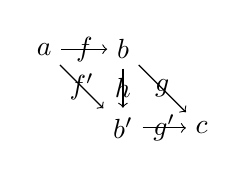
\begin{tikzpicture}
          \node (a)                {$a$};
          \node (b)  [right of=a]  {$b$};
          \node (b') [below of=b]  {$b'$};
          \node (c)  [right of=b'] {$c$};

          \draw [->] (a)  to node        {$f$}  (b);
          \draw [->] (a)  to node [swap] {$f'$} (b');
          \draw [->] (b)  to node        {$g$}  (c);
          \draw [->] (b)  to node        {$h$}  (b');
          \draw [->] (b') to node [swap] {$g'$} (c);
        \end{tikzpicture}
      \end{center}
      \caption{}
      \label{fig:commutative-triangles}
    \end{subfigure}
    \begin{subfigure}{0.5\linewidth}
      \begin{center}
        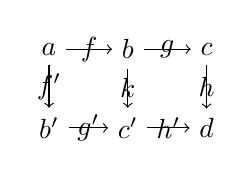
\begin{tikzpicture}
          \node (a)               {$a$};
          \node (b)  [right of=a] {$b$};
          \node (c)  [right of=b] {$c$};
          \node (b') [below of=a] {$b'$};
          \node (c') [below of=b] {$c'$};
          \node (d)  [below of=c] {$d$};

          \draw [->] (a)  to node        {$f$}  (b);
          \draw [->] (b)  to node        {$g$}  (c);
          \draw [->] (c)  to node        {$h$}  (d);
          \draw [->] (a)  to node [swap] {$f'$} (b');
          \draw [->] (b') to node [swap] {$g'$} (c');
          \draw [->] (c') to node [swap] {$h'$} (d);
          \draw [->] (b)  to node        {$k$}  (c');
        \end{tikzpicture}
      \end{center}
      \caption{}
      \label{fig:commutative-squares}
    \end{subfigure}
    \caption{Examples of commutative diagrams.}
    \label{fig:commutative-diagrams}
  \end{figure}

\end{remark}

\begin{example}
  [Trivial categories]

  %% - \parencite[10--11]{maclane-1998}
  %% - \parencite[422]{poigne-1992}

  %% - \parencite[5--6]{pierce-1991}

  \label{ex:trivial-categories}

  \catbf{0}, the empty category, is the category with no objects and
  no morphisms; \catbf{1}, the trivial category, is the category with
  one object and one (identity) morphism; and \catbf{2} is the
  category with two objects $a$ and $b$, and one nonidentity morphism
  $f: a \to b$. In each case, there is only one way to define
  composition.

  %% \catbf{0}, the empty category, is the category with no objects
  %% and no morphisms; \catbf{1}, the trivial category, is the
  %% category with one object and one (identity) morphism; \catbf{2}
  %% is the category with two objects $a$ and $b$, and one nonidentity
  %% morphism $f: a \to b$; and \catbf{3} is the category with three
  %% objects $a$, $b$, and $c$, and three nonidentity morphisms $f: a
  %% \to b$, $g: b \to c$, and $h: a \to c$. In each case, there is
  %% only one way to define composition.

\end{example}

\begin{example}
  [Discrete categories]

  %% - \parencite[11]{maclane-1998}

  %% - \parencite[422]{poigne-1992}

  \label{ex:discrete-category}

  \index{discrete category}
  \index{category!discrete ---|see{discrete category}}

  A \term{discrete category} is a category whose only morphisms are
  the identity morphisms. Given a set $A$, we get a discrete category
  \cat{C} in which $\catO{C} = A$ and $\catM{C} = \{\idO{a}: a \to a
  \mid a \in A\}$. In addition, a discrete category is determined by
  its set of objects. Thus, discrete categories are sets.

  The objects of a category correspond exactly to its identity morphisms.

\end{example}

\begin{example}
  [Sets and total functions]


  %% - \parencite[8--9, 12]{maclane-1998}
  %% - \parencite[419--420]{poigne-1992}

  %% - \parencite[26]{bird-demoor-1997}
  %% - \parencite[2]{pierce-1991}

  \label{ex:set}

  \index{\set}

  \index{function}
  \index{function!small ---}
  \index{function!total ---}
  \index{set}
  \index{set!small ---}
  \index{universe}

  Assume that there is a big enough set $U$, the \term{universe}. Then
  a set $A$ is \term{small} if it is a member of the universe.
  Similarly, a function $f: A \to B$ is small if $A$ and $B$ are
  small.
  \set is the category of all small sets and all small total
  functions. Its objects are small sets and its morphisms are small
  total functions with specified domain and specified codomain. Its
  identity function assigns to each set $A \in \catO{\set}$ an
  identity function $\idO{A}: A \to A \in \catM{\set}$ such that, for
  all $x \in A$,
  \begin{equation}
    \label{eq:set-identity}
    \idO{A}(x) = x
    \text{,}
  \end{equation}
  and its composition function assigns to each pair of functions $f: A
  \to B$ and $g: B \to C \in \catM{\set}$ a composite function $g
  \comp f: A \to C \in \catM{\set}$ such that, for all $x \in A$,
  \begin{equation}
    \label{eq:set-composition}
    (g \comp f)(x) = g(f(x))
    \text{.}
  \end{equation}

\end{example}

\begin{remark}

  \index{foundations}
  \index{universe}

  Note that our assumption of one universe is appropriate since
  considering \set as the category of all sets and all total functions
  would lead to a paradox such as the set of all sets not members of
  themselves. However, it is not necessary for us to go into detail
  about foundations of category theory.

\end{remark}

\begin{example}
  [Sets, partial functions, and relations]

  %% - \parencite[26]{bird-demoor-1997}
  %% - \parencite[420]{poigne-1992}

  \label{ex:par-rel}

  \index{\catbf{Par}}
  \index{\catbf{Pfn}|see{\catbf{Par}}}
  \index{\catbf{Rel}}

  \index{category!\catbf{Par}}
  \index{category!\catbf{Pfn}|see{\catbf{Par}}}
  \index{category!\catbf{Rel}}

  \index{function!partial ---}
  \index{relation}
  \index{set}

  Likewise, \catbf{Par} or \catbf{Pfn} is the category of all small
  sets and partial functions, and \catbf{Rel} is the category of all
  small sets and relations.

\end{example}

\begin{remark}

  \textcquote[30]{maclane-1998}{Category theory asks of every type of
    mathematical object: \enquote{What are the morphisms?}}. This
  suggests emphasizing morphisms rather than objects. However,
  category-theorists usually name categories after the common name of
  their objects---thus, \set---, but it is possible to name them after
  the common name of their morphisms---thus, \catbf{Fun}\footnote{\set
    is also known as \catbf{Fun}. See, for instance,
    \parencite{bird-demoor-1997}.}, \catbf{Par}, and \catbf{Rel}.


  %% In the
  %% case of (small) sets, \set, \catbf{Par}, and \catbf{Rel} offer three
  %% different answers: total functions, partial functions, and
  %% relations, respectively.

\end{remark}

\begin{example}
  [Monoids]


  %% - \parencite[11]{maclane-1998}
  %% - \parencite[420, 422]{poigne-1992}

  %% - \parencite[21]{adamek-2006}
  %% - \parencite[4]{pierce-1991}

  \label{ex:monoid}

  \index{monoid}

  A \term{monoid} is a category with just one object. A monoid is thus
  determined by its set of morphisms, by its identity morphism, and by
  its composition function. A monoid may then be described as a usual
  monoid, that is, as a set (of morphisms) that is closed under an
  associative binary operation, and has an identity (morphism). More
  formally, given a category \cat{C} with just one object $a \in
  \catO{C}$, we get a usual monoid $C = (\catM{C}, \comp, \idO{a})$.
  Conversely, given a usual monoid $M = (M, *, e)$, we get a category
  \cat{M} with just one object $M$ (that is, $\catO{M} = \{M\}$),
  $\catM{M} = M$, composition $*$ and identity morphism $e$.

  \index{\catbf{Mon}}

  \index{monoid}
  \index{monoid!--- homomorphism}

  Given two (usual) monoids $M = (M, *, e)$ and $M' = (M', *', e')$, a
  morphism of monoids $f: M \to M'$ is a function $f: M \to M'$ as
  described in Example \ref{ex:set} (that is, a function with
  specified domain and specified codomain) such that $f(a * b) = f(a)
  *' f(b)$ and $f(e) = e'$.

  Given two monoids $M = (M, *, e)$ and $M' = (M', *', e')$, a
  morphism of monoids $f: M \to M'$ is a function $f: M \to M'$ with
  specified domain and codomain such that $f(a * b) = f(a) *' f(b)$
  for all $a$ and $b \in M$, and $f(e) = e'$.

  \catbf{Mon} is the category of all (small) monoids, and morphisms of
  monoids or monoid homomorphisms.

\end{example}

\begin{remark}

  In general, any notion of sets with structure together with
  structure-preserving morphisms define a category
  \parencite[421]{poigne-1992}.

\end{remark}

\begin{example}
  [Monoids of strings]

  %% \parencite[420, 422]{poigne-1992}

  \label{ex:monoid-strings}

  \index{monoid}
  \index{monoid!--- of strings}
  \index{monoid!--- of words|see{--- of strings}}
  \index{monoid!free ---|see{--- of strings}}
  \index{string}
  \index{symbol}
  \index{word|see{string}}

  Given a set (of symbols) $\Sigma$, a \term{monoid of strings} (or
  \term{words}) or \term{free monoid} over $\Sigma$ is a monoid whose
  set of morphisms is the set $\Sigma^{*}$ of all strings over
  $\Sigma$, whose composition function is concatenation of strings,
  and whose identity morphism is the empty string $\epsilon$.

  %% \parencite[421]{poigne-1992}

  \index{automaton}

  In addition, automata can be defined in terms of monoids of strings,
  and automata and appropriate morphisms of automata yield categories.


\end{example}

\begin{example}
  [Preorders]

  %% - \parencite[11]{maclane-1998}
  %% - \parencite[3--4]{pierce-1991}
  %% - \parencite[421--422, 423]{poigne-1992}

  \label{ex:preorder}

  \index{category!order ---|see{preorder}}
  \index{order category|see{preorder}}
  \index{preorder}

  A \term{preorder} \cat{P}, also known as an \term{order category},
  is a category in which, for all objects $a$ and $b \in \catO{P}$,
  there is at most one morphism $f: a \to b \in \catM{P}$. Given a
  preorder \cat{P}, we define a binary relation $\leq$ on \catO{P}
  with $a \leq b$ if and only if there is a morphism $f: a \to b \in
  \catM{P}$. This binary relation is reflexive (because there is an
  identity morphism $\idO{a}: a \to a \in \catM{P}$ for all objects $a
  \in \catO{P}$) and transitive (because there is a composite morphism
  $g \comp f: a \to c \in \catM{P}$ for all morphisms $f: a \to b$ and
  $g: b \to c \in \catM{P}$). Therefore, a (usual) preorder is a set
  (of objects) equipped with a reflexive and transitive binary
  relation. Conversely, given a set $P$ with a reflexive and
  transitive binary relation $\leq$ on $P$, we get a category \cat{P}
  with $\catO{P} = P$ and $\catM{P} = \{f: a \to b \mid a \leq b\}$.
  This category has identity morphisms (because $a \leq a$ for all $a
  \in P$) and composite morphisms (because $a \leq b$ and $b \leq c$
  imply $a \leq c$ for all $a$, $b$, and $c \in P$). Equations
  \eqref{eq:category-associativity} and \eqref{eq:category-identity}
  obviously hold.

  Just like in Examples \ref{ex:set} and
  \ref{ex:monoid}, preorders and appropriate morphisms of
  preorders, that is, monotone functions, form yet another category,
  \catbf{Pre}.

\end{example}

\begin{example}
  [Deductive systems]

  %% - \parencite[5--6, 8]{marquis-2013}
  %% - \parencite[6--7]{pierce-1991}
  %% - \parencite[423]{poigne-1992}

  %% - \parencite[§ 9.1]{poigne-1992}

  \label{ex:deductive-system}

  We can look at categories as deductive systems with objects formulas
  and morphisms deductions. In this way, domains and codomains are
  premises and conclusions, respectively. A morphism is thus a proof
  of the fact that its codomain is deducible from its domain. In
  particular, identity morphisms are instances of the reflexivity
  axiom, and composition of morphisms is a rule of inference asserting
  that deductions are transitive. Note that this is just a change of
  vocabulary.

  %% Operations on morphisms are thought of as rules of inference.

\end{example}

\section{A category for Haskell}
\label{sec:category-haskell}

From the standpoint of functional programming, categories provide
important insights into types and functions, and this plays a major
role in our development. In particular, Haskell types and functions
form a category, \hask.

The objects of \hask are Haskell types, or, more precisely, nullary
type constructors or type expressions with kind \texthaskell{*} such
as \texthaskell{Bool}:
\begin{codehaskell}
data Bool = False | True
\end{codehaskell}
And \texthaskell{Maybe Bool}:
\begin{codehaskell}
data Maybe a = Nothing | Just a
\end{codehaskell}
But not \texthaskell{Maybe}, which is a unary type constructor or a
type expression with kind \texthaskell{* -> *}. However, Haskell types
have bottom. For instance:
\begin{codehaskell}
undefined :: a
undefined = undefined
\end{codehaskell}
We ignore this fact, so ``Haskell types'' means ``Haskell types
without bottom,'' which is why \hask is sometimes considered a
platonic category. Its morphisms are, of course, Haskell functions
such as \texthaskell{not}:
\begin{codehaskell}
not :: Bool -> Bool
not False = True
not True  = False
\end{codehaskell}
Its identity functions are given by the identity function:
\begin{codehaskell}
id :: a -> a
id x = x
\end{codehaskell}
And its composition function is function composition:
\begin{codehaskell}
infixr 9 .

(.) :: (b -> c) -> (a -> b) -> a -> c
g . f = \x -> g (f x)
\end{codehaskell}
As a result, the associativity and identity axioms for Haskell become
\begin{equation}
  \label{eq:hask-associativity}
  \text{\texthaskell{h . (g . f) = h . g . f = (h . g) . f}}
\end{equation}
and
\begin{equation}
  \label{eq:hask-identity}
  \text{\texthaskell{id . f = f = f . id}}
  \text{,}
\end{equation}
respectively, whenever they make sense.

\begin{proof}

  Both \eqref{eq:hask-associativity} and \eqref{eq:hask-identity}
  follow immediately from rewriting using definitions. In the first
  place:
  \begin{steps}
    \steph{(h . (g . f)) x}
      \eqbydefh{(.)}
    \steph{h ((g . f) x)}
      \eqbydefh{(.)}
    \steph{h (g (f x))}
      \eqbydefh{(.)}
    \steph{(h . g) (f x)}
      \eqbydefh{(.)}
    \steph{((h . g) . f) x}
  \end{steps}
  And, in the second place:
  \begin{steps}
    \steph{(id . f) x}
      \eqbydefh{(.)}
    \steph{id (f x)}
      \eqbydefh{id}
    \steph{f x}
      \eqbydefh{id}
    \steph{f (id x)}
  \end{steps}

\end{proof}

From now on, we will use \hask as described above as Haskell's
category\footnote{Note that this is not an attempt to answer the
  question of Haskell's category.}.

%% Note, however, that this is not an attempt to answer the actual
%% question of Haskell's category.

\section{A category for Agda}
\label{sec:category-agda}

Agda small types and functions form a category analogous to \hask, the
category of Haskell types and functions (see Section
\ref{sec:category-haskell}). The objects and morphisms of this
category are Agda small types, that is, \textagda{Set}, and functions,
respectively. Its identity functions are given by the identity
function defined in \module{Abel.Function}:
\begin{codeagda}
id : {A : Set} → A → A
id x = x
\end{codeagda}
And its composition function is function composition as defined in
\module{Abel.Function}:
\begin{codeagda}
infixr 9 _∘_

_∘_ : {A B C : Set} → (B → C) → (A → B) → A → C
g ∘ f = λ x → g (f x)
\end{codeagda}
Unlike in Haskell, the associativity and identity axioms for this
category are proved in \module{Abel.Function.Category}:
\begin{codeagda}
associativity : {A B C D : Set} {f : A → B} {g : B → C} {h : C → D}
                (x : A) → (h ∘ g ∘ f) x ≡ ((h ∘ g) ∘ f) x
associativity _ = refl

identity : {A B : Set} {f : A → B}
           (x : A) → (id ∘ f) x ≡ f x × (f ∘ id) x ≡ f x
identity _ = refl , refl
\end{codeagda}

From now on, we will use this category as Agda's
category\footnote{Note that this is not an attempt to answer the
  question of Agda's category.}.

\section{References}
\label{sec:categories-references}

\begin{itemize}
\item

  Although we define categories in terms of sets, as sets of objects
  and morphisms, they can be defined in many ways. For instance,
  \textcite{eilenberg-maclane-1945} defined them as aggregates of
  objects and mappings, and \textcite{maclane-1998} did it in terms of
  metacategories and in terms of sets, as sets of objects and arrows.
  Other ways include defining them as just a set of morphisms, and in
  terms of collections of morphisms or hom-sets. For more information
  on the basis of our definition, see
  \parencites[7--8,~10]{maclane-1998}[418]{poigne-1992}.

\item

  Regarding commutative diagrams, our definition is based on
  \parencites[8]{maclane-1998}[434--435]{poigne-1992}, but almost any
  reference on category theory contains an equivalent definition.

\item

  Additionally, our examples of categories are based on
  \parencites[8--9,~10--12]{maclane-1998}[§~1.2.2]{poigne-1992} and
  \parencites{pierce-1991}{bird-demoor-1997}{marquis-2013}.

  For more on categories of automata, see
  \parencite[421]{poigne-1992}.


\item

  As mentioned in Example \ref{ex:set}, considering \set as the
  category of all sets and all total functions would lead to a
  paradox. Our assumption of one universe is taken from
  \parencite[12]{maclane-1998}. See \parencite[§~I.6]{maclane-1998}
  for a full account on foundations of category theory.

\item

  Finally, for more information about categories in Haskell, including
  \hask, see \parencites[74]{elkins-2009}[49--51]{yorgey-2009}.

\end{itemize}

\clearemptydoublepage
